\documentclass[12pt,a4paper,twoside,openany]{book}
\usepackage{textcomp}
\usepackage[T1]{fontenc}
\usepackage[utf8]{inputenc}
\usepackage[italian]{babel}
\usepackage{pdfpages}
\usepackage{graphicx}
\usepackage{rotating}
\usepackage[formats]{listings}
\usepackage{caption}
\usepackage{float}
\usepackage{booktabs}
\usepackage{picture}
\usepackage{multirow}
\usepackage{pifont}
\usepackage[hidelinks]{hyperref}
%codice per mettere logo in sfondo ad ogni pagina
\usepackage{eso-pic}


\AddToShipoutPicture
{
  \put(\LenToUnit{.4\textwidth}, \LenToUnit{.5\textheight}){
\includegraphics{Immagini/logo}}%
}


\makeatletter
\newcommand{\lstuppercase}{\uppercase\expandafter{\expandafter\lst@token\expandafter{\the\lst@token}}}
\newcommand{\lstlowercase}{\lowercase\expandafter{\expandafter\lst@token\expandafter{\the\lst@token}}}
\makeatother

\lstdefinelanguage{myLang}
{
	morekeywords={
		select, from, on, where, group, by, order, sort, join, and, int, string, load, create, into, overwrite, if, table, not, exists, data, inpath, row, format, delimited, fields, terminated, by, stored, as, textfile, FROM, ON, WHERE, GROUP, BY, ORDER, SORT, JOIN, AND, INT, STRING, CREATE, LOAD, DATA, INPATH, OVERWRITE, INTO, TABLE, IF, NOT, EXISTS
	}
}

\lstset{
	language=myLang,
	basicstyle=\ttfamily,
	keywordstyle=\lstuppercase\color{blue}\bfseries,commentstyle=\color{green}\bfseries, stringstyle=\color{red},
	showstringspaces=false, frame=single, numbers=left, numbersep=5pt, numberstyle=\tiny\color{black}, breaklines=true,flexiblecolumns=true,
	inputpath=Sorgenti/,
	sensitive=false
}

%\lstset{basicstyle=\footnotesize\ttfamily\color{black}, language=C,keepspaces=true, format=C, inputpath=Sorgenti/,tabsize=2, keywordstyle=\color{blue}\bfseries,commentstyle=\color{green}\bfseries, stringstyle=\color{black}, showstringspaces=false, frame=single, numbers=left, numbersep=5pt, numberstyle=\tiny\color{black}, breaklines=true,flexiblecolumns=true}

%NOTA: Per ogni nuovo capitolo inserito: creare una cartella col nome dell'esercizio in Immagini ed inserirvi tutte le immagini relative all'esercizio. In seguito inserire il path nell'istruzione graphicspath secondo la sintassi {Immagini/NomeCartellaImmaginiEsercizio/} senza separazione con virgole. Notare lo slash dopo il nome della cartella per indicare che il nome inserito è una cartella.
\graphicspath{{Immagini/}}
\author{Andrea Scognamiglio - Mtr M63/598 \\ Cristian Tommasino - Mtr. M63/615}
\title{
	\centering
	\textbf{Influence Maximization}
}
\date{}

\pagestyle{plain}

\begin{document}
\frontmatter
\maketitle
\setcounter{page}{1}
\tableofcontents
\mainmatter
% !TEX root = ./main.tex
% !TEX encoding = UTF-8 Unicode
% !TEX program = pdflatex
% !TeX spellcheck = it_IT

\chapter{Introduction} \textit{"Yelp è un social network in cui le persone si
scambiano pareri,  opinioni e “dritte” sui posti migliori del luogo in cui
abitano e di  quelli in cui vanno per lavoro, viaggio o altri motivi."}
\footnote{Claudia Resta - Community di Yelp}\\\\
La mission di questo elaborato è
analizzare un dataset fornito da Yelp,  contenente informazioni riguardanti
differenti business, utenti ed un  loro sottoinsieme di recensioni effettuate,
al fine di individuare gli  utenti più influenti della rete.\\
 In particolare,
quello della \textbf{Influence Maximization} è il  problema di trovare un
piccolo \textit{subset} di nodi in una social  network tale da  massimizzare la
diffusione di influenza  (\textit{spread influence}).

% !TEX root = ./main.tex
% !TEX encoding = UTF-8 Unicode
% !TEX program = pdflatex
% !TeX spellcheck = it_IT

\chapter{Studio preliminare del dataset}
Il dataset iniziale è fornito di 5 differenti files in formato "\textbf{json}":
\begin{itemize}
	\item \textbf{User}: contiene informazioni riguardanti gli utenti iscritti e le loro amicizie (circa 1.1M);
	\item \textbf{Business}: contiene informazioni riguardanti i business recensiti (circa 144K);
	\item \textbf{Review}: contiene le recensioni che gli utenti hanno effettuato per i business (circa 4.1M);
	\item \textbf{Checkin}: contiene informazioni riguardanti le visite effettuate nel tempo presso i differenti business;
	\item \textbf{Tip}: contiene informazioni riguardanti i suggerimenti che gli utenti hanno lasciato ai differenti business.
\end{itemize}

\'E stata effettuata un'analisi preliminare del problema andando direttamente ad
utilizzare la piattaforma, al fine di comprenderne meglio le dinamiche di
funzionamento.\\
In particolare, ogni utente iscritto possiede una propria
pagina personale, sulla quale altri utenti possono lasciare differenti
"\textit{complimenti}".\\
Ogni utente può lasciare una recensione ed un punteggio in
\textbf{stars} ad un business che ha visitato.\\
Ogni recensione, a sua volta, può essere giudicata dagli altri utenti con tre
differenti reazioni:
\begin{itemize}
	\item \textbf{Funny};
	\item \textbf{Useful};
	\item \textbf{Cool}.
\end{itemize}
Yelp utilizza anche un criterio per definire influenti o meno i suoi utenti iscritti,
assegnando il titolo di "\textit{elite}".\\

\section{Analisi in Power BI}
Al fine di calpire al meglio le caratteristiche dei dati e, soprattutto, come
utilizzarli allo scopo della \textbf{Influence Maximization}, si è deciso di
effettuare un'analisi preliminare utilizando il tool di BI

% !TEX root = ./main.tex
% !TEX encoding = UTF-8 Unicode
% !TEX program = pdflatex
% !TeX spellcheck = it_IT

\chapter{Scelta Architetturale}
In questo capito sarà mostrata l'architettura del sistema utilizzato per
la risoluzione del problema di \textbf{Influence Maximization}. Il sistema è formato da un
livello di data-storage e un livello di elaborazione.

\section{MongoDB}
Nel livello data-storage del sistema, come da requisiti, si richiede l'utilizzo di un database
\textbf{NoSQL}.\\
Esistono diversi tipi di database NoSQL, tra cui: \textbf{chiave-valore}, \textbf{colonnari},
\textbf{graph-db} e \textbf{documentali}.\\
Nel caso in esame, dopo aver visionato i dati a disposizione, si scelto
un database documentale, in particolare \textit{\textbf{MongoDB}}.\\
I database documentali sono adatti alla memorizzazione di dati aggregati, ma non
adatti all'esecuzione di query complesse.\\
Infatti in tali database ogni record è visto come un documento contente delle
caratteristiche, il cui accesso è possibile
solo tramite chiave.\\
Poiché i dati forniti da \textit{Yelp} sono memorizzati in file .json che presentano
delle strutture dati complesse, come ad esempio il campo \textit{Elite} del file
utenti (contenente un array di anni), ed avendo scelto
di non effettuare processing dei dati al livello database, il db più adatto è
risultato essere appartenente a questa vasta famiglia.\\
MongoDB è stato installato per fini didattici su un singolo nodo, di seguito
saranno riportati i dettagli.

\begin{figure}[!htbp]
	
\includegraphics[width=.7\linewidth,keepaspectratio]{mongo.png}
  \caption{MongoDB}
  \label{}
\end{figure}

\section{Apache Spark}
\textbf{Apache Spark} è un framework open source per il calcolo distribuito.\\
Utilizza il paradigma MapReduce in memory riuscendo a raggiungere prestazioni
anche 100 volte superiori a quelle raggiunte da Hadoop.\\
Tale framework è disponibile nei seguenti linguaggi di programmazione:
\begin{itemize}
	\item \textit{\textbf{Scala}};
	\item \textit{\textbf{Java}};
	\item \textit{\textbf{Python}};
	\item \textit{\textbf{R}}.
\end{itemize}
Per poter utilizzare il framework di Apache Spark si è utilizzata la piattaforma
cloud \textbf{Databricks}, che cela tutte la fase di installazione e configurazione
del framework e rende disponibile direttamente all'utente (in versione community)
un \textit{cluster} composto da \textbf{8 core} e \textbf{6GB RAM}.
\begin{figure}[!htbp]
	
\includegraphics[width=.7\linewidth,keepaspectratio]{spark.png}
  \caption{Apache Spark}
  \label{}
\end{figure}

\subsection{Graphx}
Inoltre, per far fronte ad un'elaborazione di \textit{Influence Maximization},
si è dovuto ricorrere a delle strutture a grafi per la rappresentazioni dei nodi,
delle relazioni e per la realizzazione dell'algoritmo di \textit{Spread}.\\
A tal proposito si è fatto uso di \textbf{Graphx}, \textit{API} fornita da Apache
Spark, per la \textit{graph-parallel computation}.

\section{Archittettura}
In definitiva l'architettura del sistema scelto è così definita:
\begin{itemize}
	\item \textbf{MongoDB}: per lo storage dei dati di origine e per dei risultati;
	\item \textbf{Apache Spark}: per il pre-processing dei dati;
	\item \textbf{Graphx} la creazione del grafo e per l'implementazione dell'algoritmo
	 di \textit{Influence Maximization}.
\end{itemize}

\begin{figure}[!htbp]
	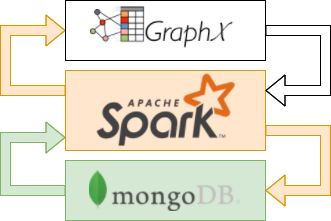
\includegraphics[width=.7\linewidth,keepaspectratio]{architettura.png}
  \caption{Archiettura del sistema}
  \label{sysarch}
\end{figure}

MongoDB è stato installato su un singolo nodo, mentre il framework Apache
Spark con le API annesse di GraphX risiedono nel cloud di Databricks.\\

% !TEX root = ./main.tex
% !TEX encoding = UTF-8 Unicode
% !TEX program = pdflatex
% !TeX spellcheck = it_IT

\chapter{Processing on Databricks}

\section{Drop dati}
In seguito è riportato il codice utilizzato per il drop di informazioni superflue
o ridondanti dai dataframe a disposizione.
\begin{figure}[!htbp]
	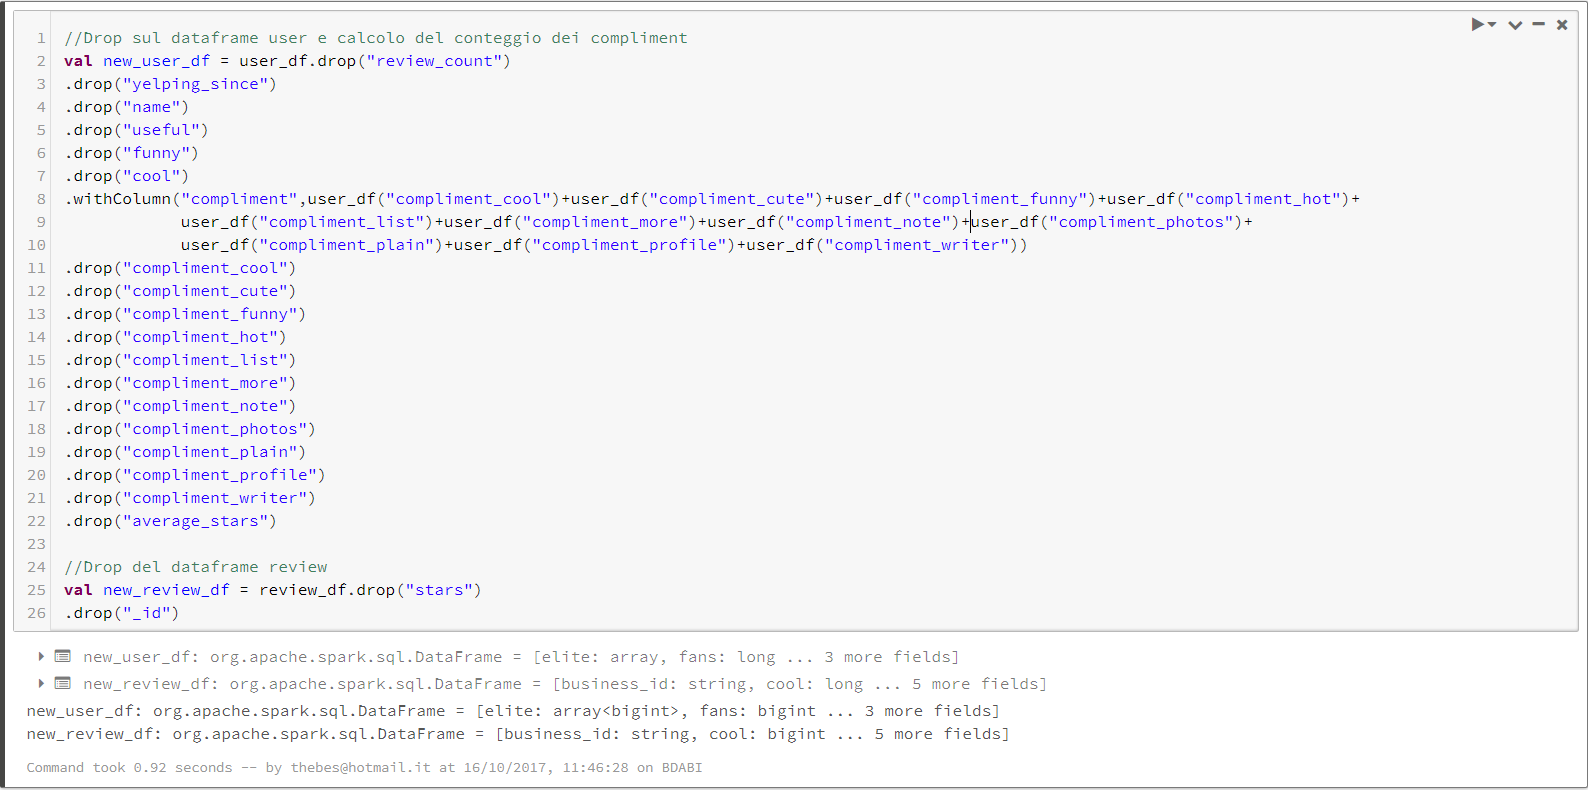
\includegraphics[width=1\linewidth,keepaspectratio]{command_1}
	\caption{Codice per il drop degli attributi superflui}
	\label{command_1}
\end{figure}

\clearpage

\section{Filtraggio Reviews}

\begin{figure}[!htbp]
	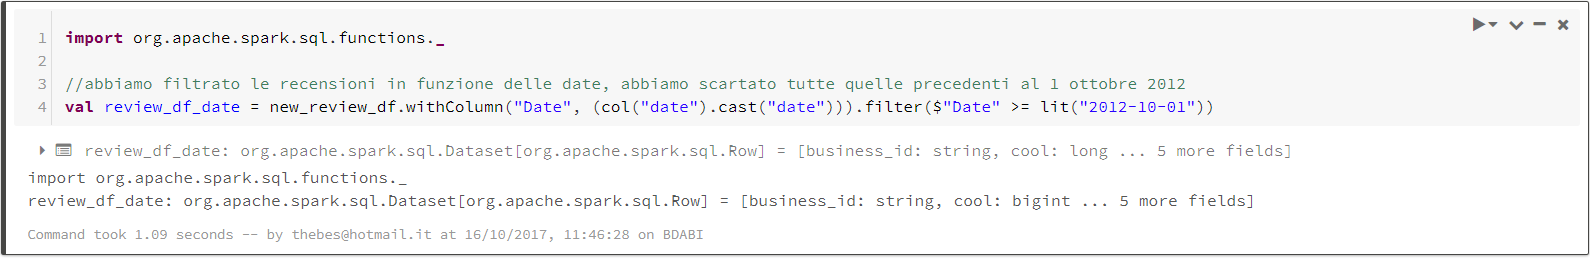
\includegraphics[width=1\linewidth,keepaspectratio]{command_2}
	\caption{Filtraggio delle reviews successive al 1 Ottobre 2012}
	\label{command_2}
\end{figure}

\clearpage

\section{Calcolo attributi di Scoring per Users}
\subsection{Creazione attributo \textit{Elite Score}}
La seguente command filtra gli utenti che hanno il titolo di ``\textit{Elite 2017}''
ed inoltre assegna loro un punteggio dato dalla somma degli anni in cui sono
stati eletti elite.
\begin{figure}[!htbp]
	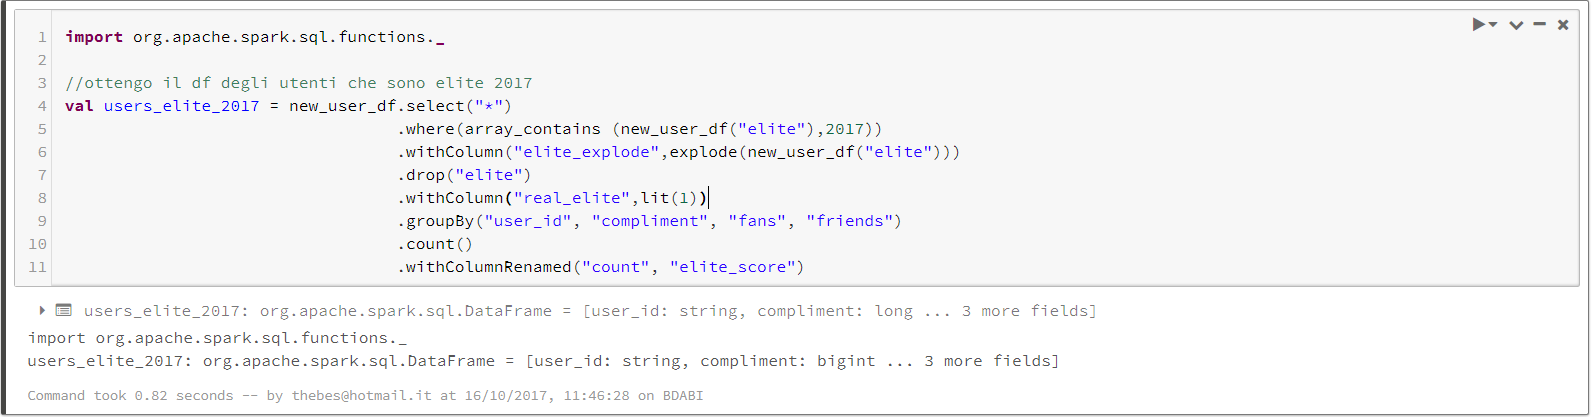
\includegraphics[width=1\linewidth,keepaspectratio]{command_3}
	\caption{Filtraggio degli utenti elite 2017}
	\label{command_3}
\end{figure}

La seguente command filtra gli utenti che non hanno il titolo di ``\textit{Elite 2017}''
ed inoltre assegna loro un punteggio nullo.
\begin{figure}[!htbp]
	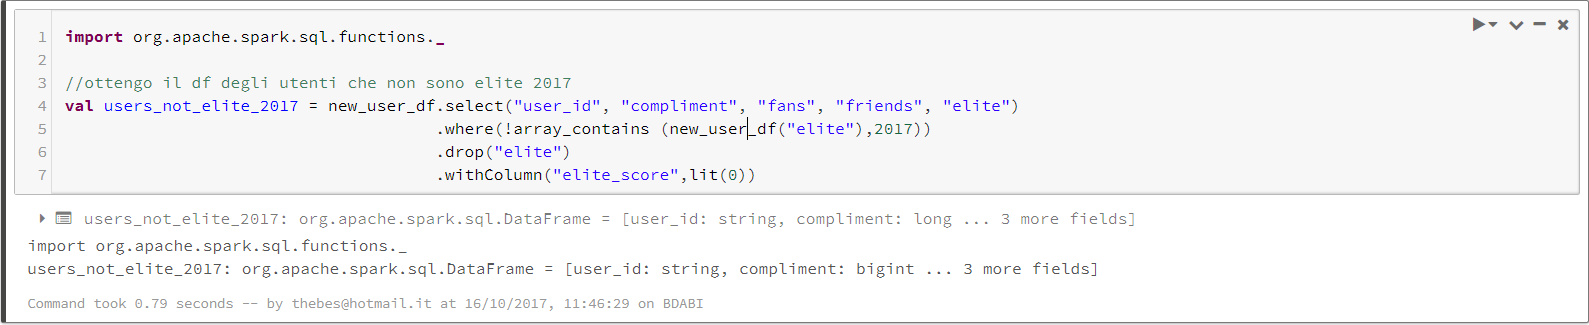
\includegraphics[width=1\linewidth,keepaspectratio]{command_4}
	\caption{Filtraggio degli utenti non elite 2017}
	\label{command_4}
\end{figure}

La seguente command crea un nuovo dataframe Users, aggiungendo il nuovo campo
numerico \textit{elite}
\begin{figure}[!htbp]
	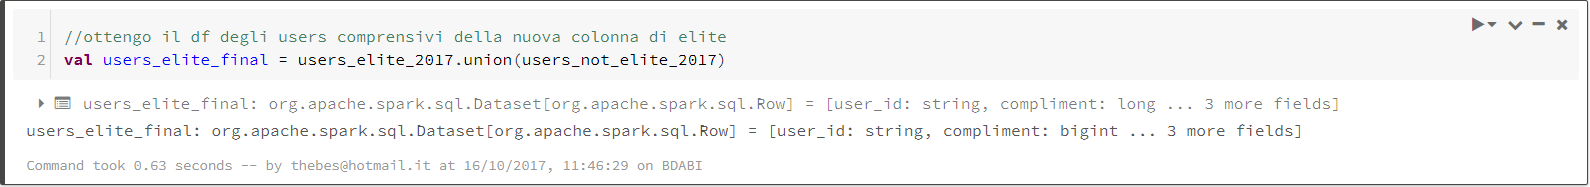
\includegraphics[width=1\linewidth,keepaspectratio]{command_5}
	\caption{Creazione dataframe users contenente il nuovo campo \textit{elite}}
	\label{command_5}
\end{figure}

\subsection{Creazione attributo \textit{Reviews Score}}
La seguente command calcola la combinazione lineare pesata degli attributi \textit{funny},
\textit{cool}, e \textit{useful}.\\
I pesi sono stati assegnati al fine di dar maggiore importanza a quelli che
sono apparsi essere più significativi per l'analisi effetuata.
\begin{figure}[!htbp]
	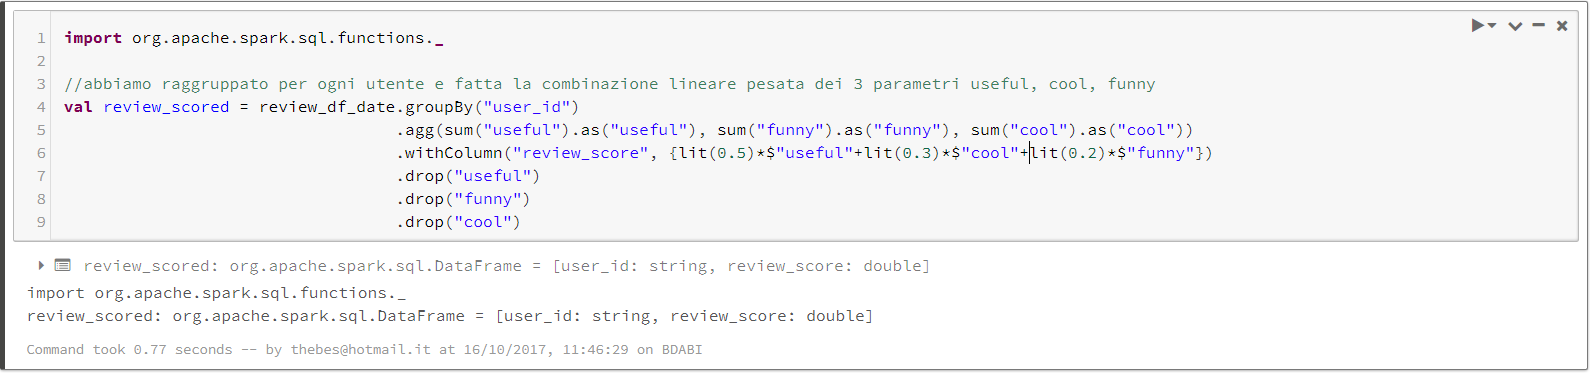
\includegraphics[width=1\linewidth,keepaspectratio]{command_6}
	\caption{Creazione attributo \textit{review\_score}}
	\label{command_6}
\end{figure}

La seguente command crea un nuovo dataframe che comprende il valore review\_score
calcolato.
\begin{figure}[!htbp]
	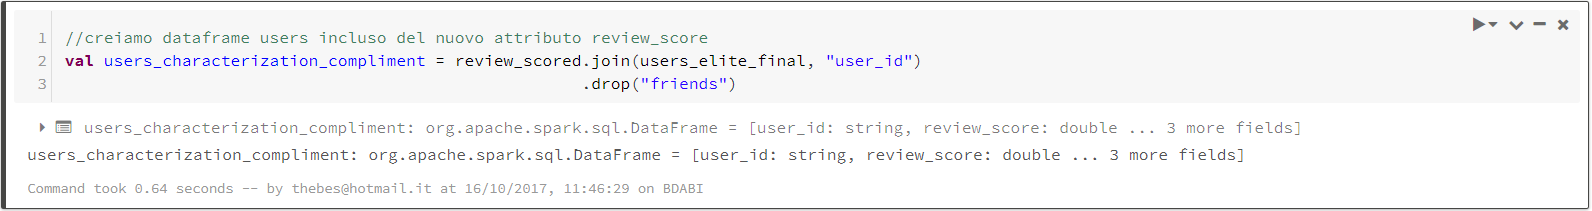
\includegraphics[width=1\linewidth,keepaspectratio]{command_7}
	\caption{Aggiunta \textit{review\_score} al dataframe users}
	\label{command_7}
\end{figure}

\clearpage

\section{Creazione dataframe relazioni user-user con peso archi}
La seguente command prepara un dataframe iniziale user\_relations in cui ogni tupla
soddisfa la proprietà che \textbf{User2} ha recensito almeno \textit{dieci}
business già precedentemente recensiti da \textbf{User1}.
\begin{figure}[!htbp]
	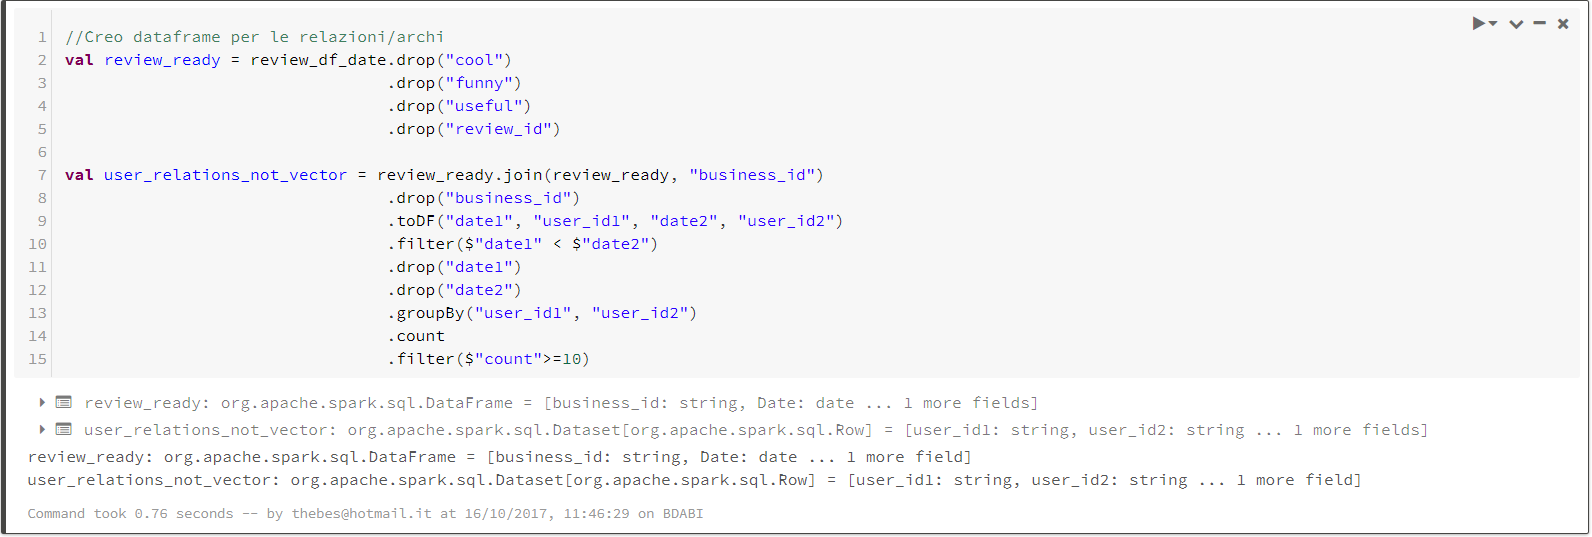
\includegraphics[width=1\linewidth,keepaspectratio]{command_8}
	\caption{Creazione dataframe user\_relations\_not\_vector}
	\label{command_8}
\end{figure}

\clearpage

La seguente command prepara i dati al fine di essere elaborati dallo
\textbf{ScalerModel}, fornito dalle librerie di machine learning di Apache Spark.\\
Questo modello permette di applicare la trasformazione \textit{Z-Score} ai dati,
al fine di normalizzarli.\\
Al termine delle operazioni della command, si ha come dataframe risultante quello
contenente \textbf{UserId1, UserId2, weight\_zscore}, ovvero le relazioni
che caratterizzeranno il grafo della Social Network.

\begin{figure}[!htbp]
	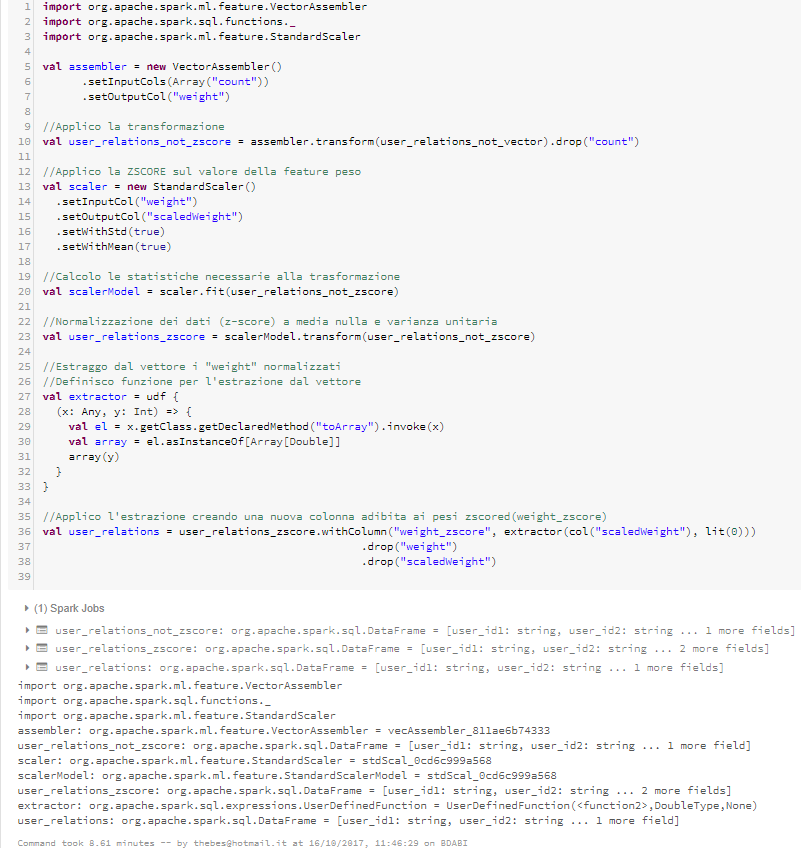
\includegraphics[width=1\linewidth,keepaspectratio]{command_9}
	\caption{Creazione dataframe user\_relations finale}
	\label{command_9}
\end{figure}

\clearpage

\section{Creazione dataframe dei vertici(users) per il grafo}
La seguente command crea un dataframe che, a partire da quello delle relazioni,
prende tutti gli users distinti, così da ottenere i vertici
del grafo.
\begin{figure}[!htbp]
	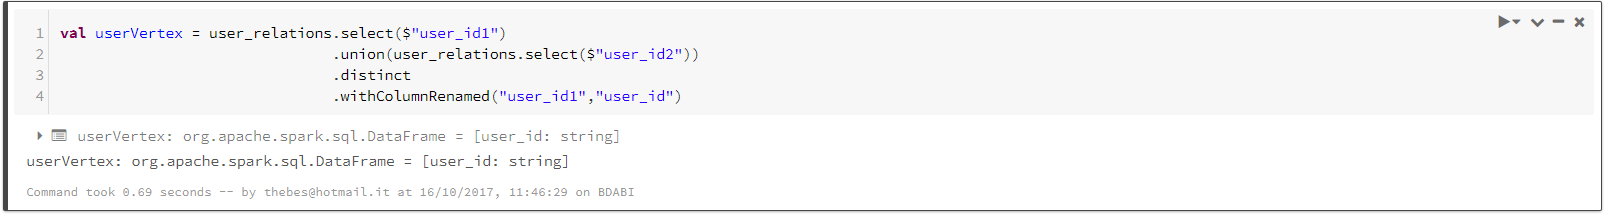
\includegraphics[width=1\linewidth,keepaspectratio]{command_10}
	\caption{Creazione dataframe user\_vertex}
	\label{command_10}
\end{figure}

Le due seguenti command preparano il dataframe per l'applicazione del modello
\textbf{ScalerModel}, al fine di normalizzare i dati prima di combinarli.\\
In seguito si estraggono le quattro \textit{features normalizzate}(review\_score,
compliment, fans, elite\_score) e se ne calcola una combinazione lineare pesata.
\begin{figure}[!htbp]
	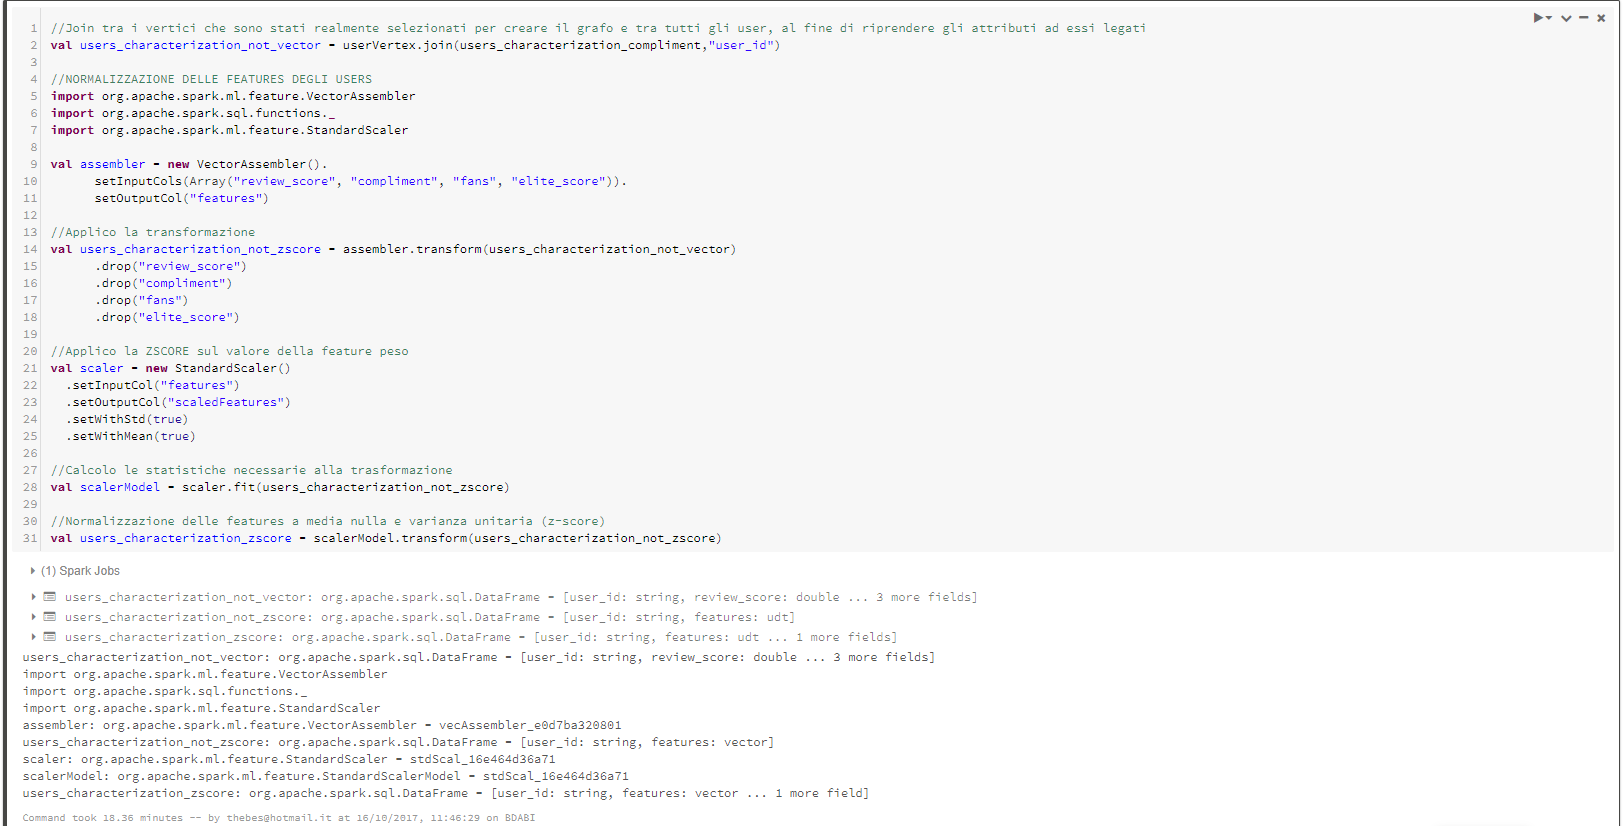
\includegraphics[width=1\linewidth,keepaspectratio]{command_11}
	\caption{Applicazione ScalerModel al dataframe user\_vertex}
	\label{command_11}
\end{figure}

\clearpage

Il risultato finale della seguente command è il dataframe che associa ad ogni user
lo score ad esso calcolato.\\
Questo score è ottenuto come media pesata delle quattro features scelte per
caratterizzare gli utenti.\\
Inizialmente, i pesi sono stati assegnati con egual valore(0.25).\\
Successivamente saranno mostrati differenti esperimenti al loro variare, al fine
di ottenere una copertura maggiore del grafo.
\begin{figure}[!htbp]
 	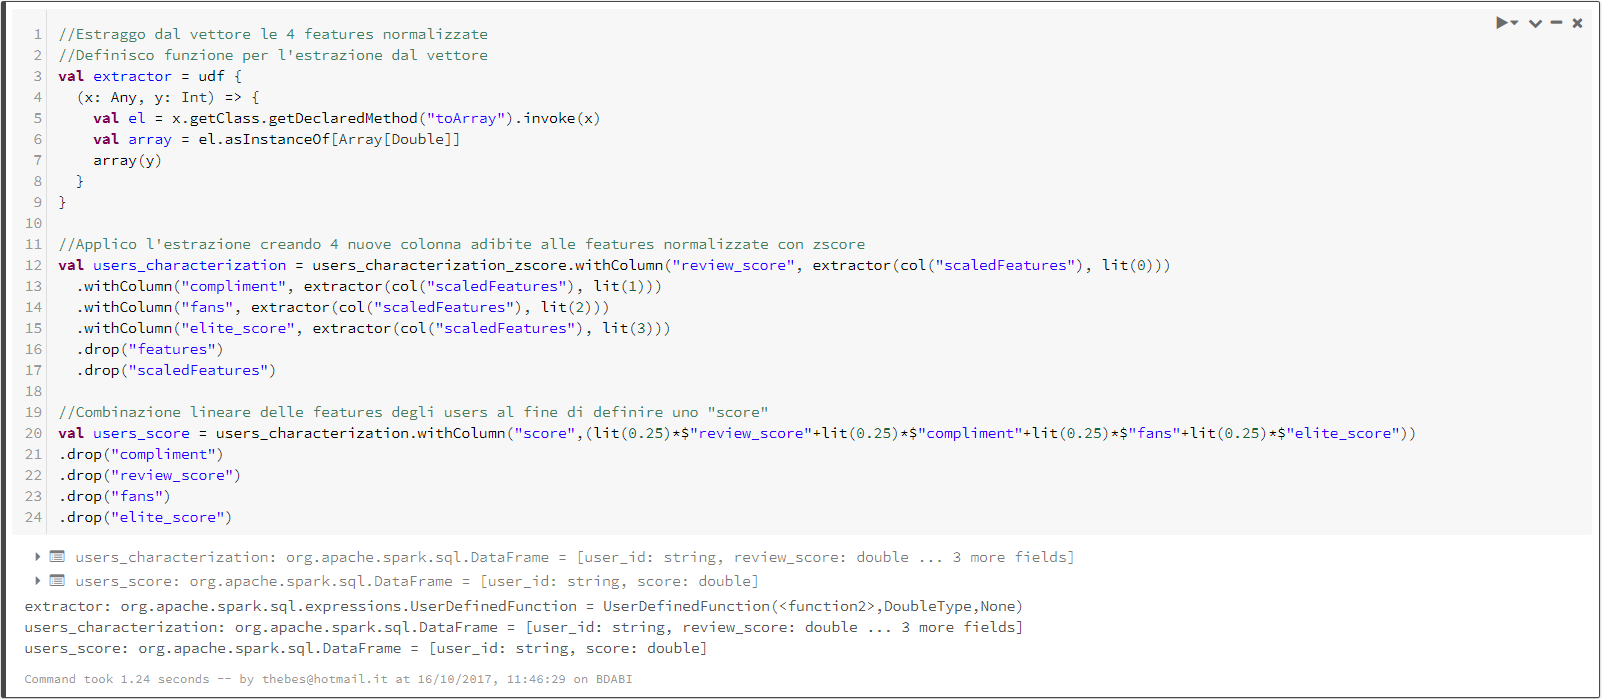
\includegraphics[width=1\linewidth,keepaspectratio]{command_12}
 	\caption{Creazione dataframe contenente user e score calcolato}
 	\label{command_12}
\end{figure}

\end{document}
